%%%%%%%%%%%%%%%%%%%%Tesis File%%%%%%%%%%%%%%%%%%%%%%%%%%%%%%%%%%%%%%%%%%%%%%%%%%%%%

\documentclass[12pt]{book}
\usepackage{cite}
\usepackage{amssymb}
\usepackage{amsthm}
\usepackage{amsmath}
\usepackage[pdftex]{graphicx}
\usepackage{setspace}
\usepackage{mathrsfs}
\usepackage{float}

%Theorems
\newtheorem{definition}{Definition}




%Commands

%Prior, posterior and likelihood
\newcommand{\post}{\mathbb{P}_{post}}
\newcommand{\like}{\mathbb{P}_{like}}
\newcommand{\prior}{\mathbb{P}_{prior}}
\newcommand{\p}{\mathbb{P}}


%Other commands
\newcommand{\E}{\mathbb{E}} %Expectation
\newcommand{\tvs}{\mathscr{T}} %TVS symbol
\newcommand{\x}{\textbf{x}}






\begin{document}
\setlength{\unitlength}{1 cm} %Especificar unidad de trabajo
\thispagestyle{empty}
\begin{center}
    %\begin{picture}(18,4)
    %\centering
    
\includegraphics[scale=0.5]{log.png} \\[1cm]
    %\end{picture}
\textbf{{\LARGE Simon Fraser University}\\[0.5cm]
{\LARGE Faculty of Sciences, Math Department}}\\[1.25cm]
\begin{doublespace}
{\huge \textbf{Here comes the title}}\\[1.5cm]
\end{doublespace}
{\large Juan Gabriel Garc{\'i}a Osorio}\\[1cm]
Advisor: John Stockie\\[1cm]
Commitee: Paul Tupper\\[1cm]
Burnaby B.C - May  2017
\end{center}

\newpage
\tableofcontents


%%%%%%%%%%%%%%%%%%%%%%%%%%%%%%%%Chapter 0 %%%%%%%%%%%%%%%%%%%%%%%%%%%%%%%%%%%%%%%%%%%%%%%%%%%%%%%
\chapter*{Acknowlegments}
\newpage


%%%%%%%%%%%%%%%%%%%%%%%%%%%%%%%Chapter 1: Introduction %%%%%%%%%%%%%%%%%%%%%%%%%%%%%%%%%%%%%%%%%%
\chapter{Introduction}

\newpage

%%%%%%%%%%%%%%%%%%%%%%%%%%%%%%Chapter 2: Theoretical and Computational Framework %%%%%%%%%%%%%%%%
\chapter{Theoretical and Computational Framework}
%\pdfmarkupcomment[markup=Squiggly,color=green]{what eve}{Change this shit}


The foundations of  our approach to estimate parameters and solve inverse problems is  the 
framework of Bayesian statistics. Unlike frequentist statistics, in the Bayesian approach, randomness
is a measure of uncertainty,  not a matter of frequency . A question like:
what is the probability of having  life in Mars? If the answer is say 0.01, in the frequentist
stastistics framework, this number is interpreted as, for every hundred times we go to 
mars under identical circumstances, one of those times we will find life there. In the Bayesian
approach the number 0.01 is interpreted as: given our current level of knowledge about mars
we think that is very unlikely that mars shelters life. Clearly there is a big philosophical
difference between these two approaches that has a direct impact in how far reaching is each point of view  \cite{jaynes2003probability}.


%Talking about Bayes rule
In real life the uncertainty associated to a  measurement or  quantity of interest is usually 
connected  with the uncertainty  of other variables involved in the problem under study. 
At this point we mention that when we talk about uncertainty we are talking about every possible 
source of randomness  or  lack of information. That is, the use of the word uncertainty in this work
is related to either epistemic (A phenomenon might not be random but the complete lack of 
understanding of it makes us see it as random) or aleatory (Inherent to the nature of phenomenon, for 
example this is the kind of randomness physicists believe is happening in quantum mechanics)
\cite{kennedy2001bayesian}.

In general the connection between the different variables is far from trivial and hard to assess.
Bayesian methodology provides a rigurous framework for the study of 
this connection, using whatever information
is available for the problem. The cornerstone of this idea
in the mathematical language is the  Bayes formula 
\begin{equation}\label{eqnBayes}
\post(A|B)=\frac{\like(B|A)\prior(A)}{\p(B)}.
\end{equation}

To explain in detail the above equation and further theory, let us first do the following two defintions
\cite{dudley2002real}
\begin{definition}\label{dfnprobabilitytriple}
A probability space is a triple $(\Omega,\mathscr{F},\p)$, where $\Omega$ is a set called 
sample space.
The element $\mathscr{F}$ is a subset of the power set of $\Omega$ that satisfies
\begin{enumerate}
\item $\emptyset,\Omega\in\mathscr{F}$.
\item If $A\in\mathscr{F}$ then $A^{c}\in\mathscr{F}$.
\item If $A_{1},A_{2},\ldots \in\mathscr{F}$ then $\bigcup_{i\in\mathbb{N}}A_{i}\in\mathscr{F}$.
\end{enumerate}
A set that satisfies properties 1 to 3 is called a $\sigma-$ algebra and its elements are called
events. The map $\p:\mathscr{F}\rightarrow [0,1]$ satisfies
\begin{enumerate}
\item $\p(\Omega)=1$.
\item If $A_{1},A_{2},\ldots \in\mathscr{F}$ are pairwise disjoint, then 
\begin{equation*}
\p(\bigcup_{i\in\mathbb{N}}A_{i})=\sum_{i\in\mathbb{N}}\p(A_{i}).
\end{equation*}
\end{enumerate}
$\p$ is called a probability measure. 
\end{definition}
Another important notion is given by
\begin{definition}\label{dfnrandonvariables}
Given a probability space $(\Omega,\mathscr{F},\p)$, a function $X:\Omega\rightarrow\mathbb{R}$ is called 
a random variable
if $X^{-1}(C)\in\mathscr{F}$ for all $C$ in the $\sigma$-algebra generated by the open sets of $\mathbb{R}$.
 An $n$-dimensional random vector $\textbf{X}=(X_{1},\ldots,X_{n})$ is a function 
$\textbf{X}:\Omega\rightarrow\mathbb{R}^{n}$, such that each component is a random variable. The 
distribution of a random vector is the probability measure $\p\circ \textbf{X}^{-1}$. If for any 
$C$ in the $\sigma$-algebra generated by the open sets in $\mathbb{R}^{n}$ we have
\begin{equation}\label{eqnmultivariateGaussianDefinition}
(\p\circ\textbf{X}^{-1})(C)=\int_{C}
\frac{1}{2\pi det(\Sigma)^{-\frac{1}{2}}}\exp((\textbf{x}-\textbf{x}^{*})^{T}\Sigma^{-1}
(\textbf{x}-\textbf{x}^{*}))d\textbf{x},
\end{equation}
then we say
that $\textbf{X}$ has multivariate normal distribution with mean $\textbf{x}^{*}\in\mathbb{R}^{n}$
and covariance matrix $\Sigma$, where $\Sigma$ is symmetric positive definite matrix. We shall write
\begin{equation}\label{eqnMultivariate}
\textbf{X}\sim \mathcal{N}(\textbf{x}^{*},\Sigma).
\end{equation}
In this case the components of $\textbf{X}$ are said to be \textit{joinly Gaussian}.
\end{definition}


%In equation (\ref{eqnBayes}), $\p,\prior,\like,\post$ are different probability measures defined in the
%same sample space $\Omega$. 
The sets $A$ and $B$ are subsets of the sample space $\Omega$ and 
are elements of the associated $\sigma-$algebra $\mathscr{F}$. The bar in the probability
measures e.g. $\like(\cdot|\cdot)$, means conditional probability. Let us introduce some terminology:
 the term $\like(B|A)$ is called the \textit{likelihood} of $B$ given $A$, $\prior(A)$ is called the 
\textit{prior} probability for $A$. The prior expreses how much we believe the event $A$ to happen without assuming
anything about how the event $B$ might influence the event $A$. 
The term $\p(B)$ is a \textit{normalization constant} defined as 
\begin{equation*}
Z=\int_{\Omega} \like(B|A)\prior(A)d\p.
\end{equation*}
The term $\post(A|B)$ is  the \textit{posterior}. The posterior contains all the information 
gained when comparing our beliefs (contained in the prior) with experimental data (likelihood). 
Simply put  formula (\ref{eqnBayes}) implies: the probability that the event $A$ given that
the event $B$ has already occurred is proportional to the probability of the event $B$ given
that the event $A$ has already happened weighted by the prior probability of $A$.
\newline



%Ilustratory example
This interpretation of Bayes rule serves as a motivation for using it in the field of inverse problems. 
Inverse problems are  of the type `find the cause of this effect'. This name is relative to what is known
as the forward problem. Forward problems are  of the type `find the effect of this cause'. That is why
the posterior
is the \textit{solution of an inverse problem} when using the  Bayesian framework.
Often, inverse problems
are ill-posed, this means
that these problems might  not satisfy one or more of the following properties \cite{lebedev2012functional}:
\begin{itemize}
\item Existence: There exists a solution for the problem.
\item Uniqueness: The problem has a unique solution.
\item Stability: Small changes in inputs result in small changes in outputs.
\end{itemize}
This is a serious issue. If the problem under study has at least one solution but  is not stable, for example, 
how can we assess the accuracy of the result obtained? Therefore an statistical approach is called for 
. The reason why the Bayesian framework is useful to solve inverse problems
is that Bayes rule unifies the problem of `find the cause of this effect' (e.g. finding the posterior)
with the direct problem of `find the effect of this cause' (e.g. finding the likelihood).

Let us be precise of how the Bayesian approach can be used to solve inverse problems with an example. 
Consider the problem of finding the location where a rock that smashed a window was thrown. We can
start by considering the following events
\begin{center}
$A$=x,y,z coordinates where the rock was thrown.\\
$B$=x,y,z coordinates where the rock hit the window.
\end{center}
In this case Bayes formula  tells us that if we want to estimate the likely locations  where the rock was 
thrown from (find the posterior probability), given that we 
know the coordinates where it hit the window we need to include our prior believe on where
do we think the rock was actually thrown (Setting a prior probability). Also it is necessary
to find the connection with the forward problem. In this case the forward problem is to estimate where
the rock hit the window assuming that we know where it was thrown (find the likelihood probability) 
\newline



Let us evaluate how we could estimate the different probabilities mentioned in the previous paragraph. 
First, to find the likelihood
we need to know how the rock's impact position  in the window  is related to the launch location 
. If we treat air resistance as a source of uncertainty  we can use
the kinematics equations  for parabolic trajectories to get \cite{arnol2013mathematical}
\begin{equation}\label{eqnKinematics}
\textbf{r}=\textbf{r}_{0}+\textbf{v}_{0}t+\frac{1}{2}\textbf{g}t^{2},
\end{equation} 
where $\textbf{r}$ and $\textbf{r}_{0}$ are the final and initial position of the rock respectively, 
$\textbf{v}_{0}$ is 
the initial velocity  and $\textbf{g}$ is  a vector that points to the center of the earth and has a 
magnitude equal to the value of the gravity. The scalar $t$ represents time.
In a more physical language, to estimate the likelihood it is necessary to estimate $\textbf{r}$ (where the 
rock hit the window) assuming we know $\textbf{r}_{0}$ (where it was thrown). 
To do so,
we  need to estimate the initial velocity of the rock $\textbf{v}_{0}$. 
Once all the other variables are identified the value of $t$ can be computed in a straightforward manner. 

Equations in physics are just models of reality and as such are just an approximation to it. To take
this into account we add an extra layer to the model by adding a random parameter that accounts
for the discrepancy of our model. We propose 
\begin{equation*}
\textbf{r}=\textbf{r}_{0}+\textbf{v}_{0}t+\frac{1}{2}\textbf{g}t^{2}+\mathbf{\epsilon},
\end{equation*} 
where $\mathbf{\epsilon}$ is a random vector distributed as $\vec{\epsilon}\sim\mathscr{N}(0,\sigma I)$. Here $I$
represents the $3\times 3$ identity matrix and $\sigma>0$ parametrizes one belief in quantifying the 
accuracy  
of equation (\ref{eqnKinematics}).  By introducing a random variable into the model
we make all variables involved  in equation (\ref{eqnKinematics})
to be  random variables, that is, we now look at the  associated stochastic equation. With this notation
we can cast equation (\ref{eqnBayes}) into  (assuming independence between $\textbf{r}_{0}$ and $\textbf{v}_{0}$)
\begin{equation}\label{eqnpostrock}
\post(\textbf{r}_{0}|\textbf{r},\textbf{v}_{0})=\frac{\like(\textbf{r}|\textbf{r}_{0},\textbf{v}_{0})
\prior(\textbf{r}_{0})}{\p(\textbf{r}|\textbf{v}_{0})}.
\end{equation}



Since $\mathbf{\epsilon}$ is Gaussian we can readily obtain \cite{Somersalo}
\begin{equation*}
\textbf{r}|\textbf{r}_{0},\textbf{v}_{0}\sim \mathscr{N}(\textbf{r}_{0}+\textbf{v}_{0}t+\frac{1}{2}\textbf{g}t^{2}
,\sigma I),
\end{equation*}
This equation gives an explicit density for the likelihood. We now turn our attention to model the prior.
Suppose that we suspect that the rock was thrown from the bedroom of one of our neighbors.
 One way to model this suspicion is to assume a prior distribution on $\textbf{r}_{0}$ as
\begin{equation*}
\textbf{r}_{0}\sim\mathscr{N}(\textbf{z},\lambda I),
\end{equation*}
where $\textbf{z}$ is the coordinate vector of the center of mass of our neighbor's room and $\lambda$ represents 
the variance of the launch location around the point $\textbf{z}$. We note that  this is one way to model 
 prior knowledge and other priors are also possible for our problem.

The last quantity to find is   the normalization constant $\p(\textbf{r}|\textbf{v}_{0})$. Since all
probabilities  are normalized, if we integrate over the whole space equation (\ref{eqnpostrock}), we get
\begin{eqnarray*}
1=\int_{\mathbb{R}^{3}}\post(\textbf{r}_{0}|\textbf{r},\textbf{v}_{0})d\textbf{r}_{0}\\
=\int_{\mathbb{R}^{3}}\frac{\like(\textbf{r}|\textbf{r}_{0},\textbf{v}_{0})
\prior(\textbf{r}_{0})}{\p(\textbf{r}|\textbf{v}_{0})}d\textbf{r}_{0}.
\end{eqnarray*} 
Since the denominator in the last integrand is  constant with respect to the variable of integration 
we conclude
\begin{equation*}
\p(\textbf{r}|\textbf{v}_{0})=\int_{\mathbb{R}^{3}}\like(\textbf{r}|\textbf{r}_{0},\textbf{v}_{0})
\prior(\textbf{r}_{0})d\textbf{r}_{0}.
\end{equation*}


Having the likelihood, prior and normalization constant allow us to compute the posterior using
Bayes rule. Note that the posterior is a probability density so in order to obtain useful
statistics,  is necessary to sample from it. How to sample from a probability density is going
to be explained in the next chapter. For the moment assume we have the means to sample from the 
posterior in equation (\ref{eqnpostrock}). By having samples from the posterior we can obtain
pointwise estimates of the parameters of interest. Common choices of pointwise estimates
include
\begin{eqnarray*}
\textbf{r}_{MAP}=argmax_{\textbf{r}_{0}}\post(\textbf{r}_{0}|\textbf{r},\textbf{v}_{0}). 
\qquad\text{(Maximum a posteriori)}\\
\textbf{r}_{CM}=\int_{\mathbb{R}^{3}}\textbf{r}_{0}\post(\textbf{r}_{0}|\textbf{r},\textbf{v}_{0})d\textbf{r}_{0}.
\qquad\text{(Conditional mean)}. \\
\textbf{r}_{ML}=argmax_{\textbf{r}_{0}}\post(\textbf{r}_{0}|\textbf{r},\textbf{v}_{0}).
\qquad\text{(Maximum likelihood)}
\end{eqnarray*}

Each  of these estimates have strengths and weaknesses. If the posterior is bimodal, then the conditional
mean might point at a value with very low probability, whereas the maximum a posteriori might be more 
reliable. If the posterior has no critical points then the mean might be use as a point estimate. We can 
also assess how confident we are about the point estimate. If $\textbf{r}^{*}$ is our point
estimate we can calculate $\alpha>0$ such that
\begin{equation*}
\int_{B(\textbf{r}^{*},\alpha)}\post(\textbf{r}_{0}|\textbf{r},\textbf{v}_{0})d\textbf{r}_{0}=0.95,
\end{equation*}
where $B(\textbf{r}^{*},\alpha)$ is a ball centered at $\textbf{r}_{0}$ and radius $\alpha$. This 
uncertainty estimate can be thought of  the Bayesian version 
of the frequentist's $95\%$ confidence interval.
Another way to estimate the uncertainty is by calculating the covariance matrix as
\begin{equation*}
\int_{\mathbb{R}^{3}}(\textbf{r}-\textbf{r}^{*})\otimes(\textbf{r}-\textbf{r}^{*})d\p,
\end{equation*}
\newline
and then the diagonal of this matrix is going to contain the variance on each of the variables.
We solved our mystery, we have a way to estimate where the rock was thrown and a way to measure how
confident we are about this estimate. 
\newline


%Caveats of computing complex models
Practical problems are often substantially more challenging than the above example. Often times we have to 
deal with several issues such as 

\begin{enumerate}
\item Uncertainties in experimental measurements.
\item Lack of sufficient information and data.
\item Computational complexity of  physical models that are too expensive to evaluate.
\item Parameters of interest belong to high dimensional spaces so the associated probability density is 
hard to sample from.
\item Evaluating any of the possible point estimates for the quantity of interest might be very hard.
\end{enumerate}
In the problem described in the Chapter 1, we have to deal with the above mentioned issues.
In this chapter we are going to discuss our approach to deal with issues 3, 4 and 5 above. We 
omit 1 and 2, since these  are intrinsic in the physics of the problem and   the methodology used 
to obtain the experimental data, both of these aspects are out of our hands.


%%%%Dealing with computational complexity
\section{Dealing with  the computational complexity of the physical model}
Models of physical processes are often complex and are  expensive to simulate numerically.
Following O'Hagan  \cite{o2006bayesian}, we think of our  mathematical model of the physical process
 as a function
$M(\cdot)$ that takes a vector $\textbf{x}$ of inputs and gives back a vector $\textbf{y}$ of outputs.
For simplicity we will assume that the output is an scalar and not a vector.  
Mathematical models are approximations to explain the reality and as such there is uncertainty associated
to them. Since mathematical models are expensive,
this means that estimating the uncertainty via   classical methods such  as in 
\cite{saltelli2000sensitivity} is not feasible. Here the concept of emulator as defined in \cite{o2006bayesian} 
comes into play. We 
approximate the function $M(\cdot)$, which is assumed to be expensive to evaluate,
 with a function $\hat{M}(\cdot)$ that is cheaper. To construct an approximation,   
we  associate a 
probability distribution to each  possible value of $M(\textbf{x})$ and then take the mean
of this distribution as  $\hat{M}(\textbf{x})$, for example. We will call such approximation $\hat{M}(\cdot)$ and emulator. 
Following \cite{o2006bayesian} we create the emulator in the following steps 
\begin{itemize}
\item At points $\textbf{x}$  were we know the output of the mathematical model i.e. $M(\textbf{x})$,
the emulator should satisfy $\hat{M}(\textbf{x})=M(\textbf{x})$.
\item For  points $\textbf{x}^{*}$ where we don't know the output $M(\textbf{x}^{*})$, the emulator should
give back an estimate $\hat{M}(\textbf{x}^{*})$, based on the distribution for $M(\textbf{x}^{*})$. 
That estimate should reflect the uncertainty associated with
the interpolation/extrapolation done at that point.
\end{itemize} 

From now on in this work we are going to refer to the mathematical model or the computationally expensive
function to calculate as $M$. The emulator that approximates this function is going to be denoted by $\hat{M}$.
%Talking about Gaussian processes

A very popular  method to produce an emulator with the desired
extrapolation/interpolation properties is what is known as a Gaussian Process, we will discuss this topic next.  

\subsection{Gaussian Processes}
The conditions we need to get an emulator $\hat{M}(\cdot)$ as stated above imply that we need
to work with a probability distribution for each point $\textbf{x}$ in the domain of the emulator.
This means that  we need
to deal with a very big (probably uncountable) number of random variables. When dealing with 
several random variables there is one probability density that is computationally tractable and
easy to work with: the multivariate Gaussian distribution. The density for this distribution
is given in Definition \ref{dfnrandonvariables}. 


The computational advantages
when working with a random vector distributed as in  
equation ($\ref{eqnmultivariateGaussianDefinition}$) motivates the following definition.

\begin{definition}\label{dfnGP}
A Gaussian process (GP) is a collection of random variables $\{g(x)\}_{x\in A}$, for some set $A$, 
possibly uncountable,
 such that any finite subset of random variables
 $\{g(x_{k})\}_{k=1}^{N}\subset\{g(x)\}_{x\in A}$ for 
$\{x_{k}\}_{k=1}^{N}\subset A$ are jointly Gaussian
\cite{rasmussen2006gaussian}. 
\end{definition}

A GP is specified by a mean function and a covariance operator or kernel. 
Following  Rasmussen \cite{rasmussen2006gaussian} we define
\begin{eqnarray*}
m(x):=\E(g(x)),\qquad\text{(Mean)}\\
k(x,x'):=\E((g(x)-m(x))(g(x')-m(x')))\qquad\text{(Kernel)}.
\end{eqnarray*}
If $\{g(x)\}_{x\in A}$ is a GP with mean $m(x)$ and covariance $k(x,x')$ we will write
\begin{equation*}
g(x)\sim \textbf{GP}(m(x),k(x,x')).
\end{equation*} 

To understand the notion of a GP, recall that our goal is to create
an emulator $\hat{M}(\cdot)$ that approximates a function $M(\cdot)$. 
For a fixed $x\in A$, a realization of the  random variable $g(x)$ represents
a possible value of $M(x)$. The mean function at that point $x$, i.e. $m(x)$ 
represents the best prediction about the true value of $M(x)$. We may set
$\hat{M}(x)=m(x)$. Later we will show that the uncertainty 
associated to that prediction is given by the quantity $k(x,x)$.

 

We are going to use GPs to fit  functions in  high dimensional euclidean space, therefore from 
here on we thing 
of the set of index set $A$ in definition \ref{dfnGP} as $\mathbb{R}^{n}$ for some $n\geq 1$. 
\newline

The reason why the definition  Gaussian processes is useful in practice is that  GPs are 
completely characterized by $m(x)$ and $k(x,x')$\cite{lifshits2012lectures}. 
 For example a  common covariance or kernel is the
 squared exponential (SE) function
\begin{equation}\label{eqnsquareexponential}
k(x,x')=e^{-\frac{1}{2}\|x-x'\|_{2}^{2}}.
\end{equation}
The reason to use the name squared exponential instead of Gaussian is to avoid confusion with
the probability distribution.
This  covariance function tells us that points that are close to each other
are highly correlated whereas far away points have a correlation that decays exponentially fast.
There are some `standard' ways to choose the covariance function depending on the kind
of regularity we want for the realizations of the GP.
Some of the most common kernels are \cite{rasmussen2006gaussian} (setting $r=\|x-x'\|_{2}$)

\begin{itemize}
\item Squared-Exponential: $k(r;\theta)=e^{-\frac{1}{2}(\frac{r}{\theta})^{2}}$
\item Exponential: $k(r;\theta)=e^{-\frac{r}{\theta}}$\\
\item Matern $\frac{3}{2}: k(r;\theta)=(1+\frac{\sqrt{3}r}{\theta})e^{-\frac{\sqrt{3}r}{\theta}}$.
\item Matern $\frac{5}{2}: k(r;\theta)=(1+\frac{\sqrt{5}r}{\theta}+\frac{5}{3}
(\frac{r}{\theta})^{2})e^{-\frac{\sqrt{5}r}{\theta}}$.
\item Power-Exponential: $k(r;\theta,p)=e^{-(\frac{r}{\theta})^{p}}$.
\end{itemize}

Mathematically, GPs are measures on function spaces. We now discuss them in this
context following \cite{lifshits2012lectures}.




\subsubsection{Distributions Over Function Spaces}
Interesting function spaces (e.g. $L^{p}$ spaces, Sobolev spaces, etc...) are 
normed vector spaces, with a topology inherited from the metric induced by the norm, and so 
, function spaces are topological vector spaces (TVS). 

Let $\mathscr{T}$ be a TVS and  let $\mathscr{T}^{*}$ be its topological dual. 
We will denote the action of an 
element $h\in\tvs^{*}$ over an element $z\in\tvs$ with $\langle h,z\rangle$. Moreover 
we  define a random variable taking values in $\tvs$ as a map 
\begin{equation*}
X:(\Omega,\mathscr{F},P)\longrightarrow\tvs,
\end{equation*}
that is measurable with respect to the $\sigma$-algebra generated by the topology
of $\tvs$. This $\sigma$-algebra is known as the Borel $\sigma$-algebra for $\tvs$.
The triple $(\Omega,\mathscr{F},P)$ is a probability space as in definition \ref{dfnprobabilitytriple}. 
We use the shorthand notation  $X\in\tvs$ whenever the random variable $X$ takes vales in $\tvs$. 
For example if $\tvs=L^{2}(\mathbb{R})$,  then  $X\in L^{2}(\mathbb{R})$ means that $X$ is a measurable
map from the probability space $(\Omega,\mathscr{F},P)$ into $L^{2}(\mathbb{R})$.

We say that a random variable $X\in\tvs$ is called Gaussian if $\langle h,X\rangle$ is
a Gaussian random variable on the real line for all $h\in\tvs^{*}$. We say that an element $a\in\tvs$ is the 
expectation of $X\in\tvs$ if 
\begin{equation*}
\E(f,X)=\langle f, a\rangle,\qquad\text{for all }f\in\tvs^{*}.
\end{equation*}
Also a linear and positive definite operator $K:\tvs^{*}\longrightarrow \tvs$ 
is called the covariance operator (e.g. covariance
matrix in the finite dimensional case) if
\begin{equation*}
cov(\langle f_{1},X\rangle,\langle f_{2},X\rangle)=\langle f_{1},Kf_{2}\rangle,
\end{equation*}
for all $f_{1},f_{2}\in\tvs^{*}$. In this case we say that $X$ is distributed as 
$\mathcal{N}(a,K)$ if  $X$ is Gaussian with mean $a$ and covariance operator $K$. It is worth mentioning
that given a covariance operator $L$ and an element $b\in\tvs$ the distribution $\mathcal{N}(b,L)$
does not always exist. But if it does exist, to define the  Gaussian measure $\mathcal{N}(a,K)$, it is
only necessary to know $a$ and $K$.
\newline

%%%%%%%%%%%%%%%%%%%%%%%Think about this bit %%%%%%%%%%%%%%%%%%%%%%%%%%%%%%%%%%%%%%%%%%%%%%%%%%%%%%
%with the construction of a rigorous framework that allows us to talk about gaussian distributions in 
%function spaces we can see why once the covariance function and the mean function are defined then we 
%have created a Gaussian distribution over some function of spaces and why the nature of the function
%space depends heavily on the regularity properties of the covariance kernel. 

%%%%%%%%%%%%%%%%%This is also you need to think about %%%%%%%%%%%%%%%%%%%%%%%%%%%%%%%%%%%%%%%
%%%%%%%%%%%%%%%%%%%%What is the connection between K and a covariance function k(x,x')?%%%

%In this work we are going to be mainly concerned to work with kernels that are at least continuous
%(For example the SE kernel in equation (\ref{eqnsquareexponential}) is $C^{\infty}$). 
As an example consider the  $\tvs=\mathbb{C}(T)$ where 
$T\subset\mathbb{R}^{n}$ and $T$ is compact. This is the  space of real valued continuous functions 
defined in 
$T$. This  is a Banach
space with the norm \cite{bressan1900lecture}
\begin{equation*}
\|h\|=\max_{x\in T}|h(x)|.
\end{equation*}
The dual space of $\tvs$ is given by $\tvs^{*}=\mathbb{M}(T)$ the set of signed measures defined on 
the borel $\sigma-$ algebra of  $T$. In this 
case the duality pairing is given by 
\begin{equation*}
\langle\mu,g \rangle=\int_{T}gd\mu.
\end{equation*}
Given a GP,  $\{g(t)\}_{t\in T}$ (see definition \ref{dfnGP}) with mean function $m(t)$ and 
covariance kernel $k(t,t')$, it can be thought as a Gaussian measure $\mathcal{N}(m,K)$
where
\cite{lifshits2012lectures} 
\begin{eqnarray*}
\E(f)=m\in\mathbb{C}(T), \\
(K\nu)(t)=\int_{T}k(t,t')\nu(dt'),\qquad\text{for }\nu\in\mathbb{M}(T).
\end{eqnarray*}

The above example shows the connection between GPs and distribution over function spaces. More
precisely how it is connected to Gaussian measures in function spaces. Now we move on
into explaining how to use GPs in a practical setting.

Assume  we have some  results  (training inputs) from an expensive function to evaluate $M(\cdot)$, 
$\{(\textbf{x}_{i},y_{i})\}_{i=1}^{m}\subset\mathbb{R}^{n}\times\mathbb{R}$, where $M(\textbf{x}_{i})=y_{i}$. For
simplicity we assume no trend in the training inputs. Given this data 
we would like to infer  possible values of $M(\cdot)$ on another set of points 
$\{\textbf{x}_{j}^{*}\}_{j=1}^{k}$ (test inputs),
by creating an emulator $\hat{M}(\cdot)$ (see introduction to section 2.1).
To construct $\hat{M}(\cdot)$  we  use the GP denoted by $\{f(\textbf{x})\}$ where $\textbf{x}$ 
belongs to the domain of $M(\cdot)$.
 By
definition \ref{dfnGP}, the random vectors
\begin{eqnarray*}
\textbf{f}=\begin{bmatrix}f(\textbf{x}_{1}) & \ldots & f(\textbf{x}_{m}) \end{bmatrix}^{T}, \\
\textbf{f}^{*}=\begin{bmatrix}f(\textbf{x}_{1}^{*}) & \ldots & f(\textbf{x}_{l}^{*}) \end{bmatrix}^{T},
\end{eqnarray*}
are  jointly Gaussian, i.e. 
\begin{equation}\label{eqnconditional}
\begin{bmatrix}
\textbf{f} \\
\textbf{f}^{*}
\end{bmatrix}\sim\mathscr{N}\left(0,\begin{bmatrix} K(X,X) & K(X,X^{*}) \\
						    K(X^{*},X) & K(X^{*},X^{*}) \end{bmatrix}
\right),
\end{equation}	
The zero mean models the assumption of no trend in the data. 
Here
$(K(X,X))_{ij}=cov(f(\x^{i}),f(\x^{j})), K(X,X^{*})_{ij}=cov(f(\textbf{x}_{i}),f(\x_{j}^{*}))$ and so on.


By the requirements asked in the definition of an emulator at the beginning of section 2.1
 the realization of the random vector $\textbf{f}$ is known and should be equal to $\{y_{i}\}_{i=1}^{m}$.  
We want to make inferences about the vector $\textbf{f}_{*}$,
therefore we are looking for the distribution of $\textbf{f}_{*}|\textbf{f}$. By well known properties
of the multivariate Gaussian distribution we  obtain  \cite{lifshits2013gaussian}
\begin{equation}\label{eqnformulameancovariance}
\textbf{f}^{*}|\textbf{f}\sim\mathscr{N}\left(K(X^{*},X)K(X,X)^{-1}\textbf{f},
K(X^{*},X^{*})-K(X^{*},X)K(X,X)^{-1}K(X,X^{*})\right).
\end{equation}
Note that in the mean $K(X^{*},X)K(X,X)^{-1}\textbf{f}$ if we replace the test inputs in the matrix
$K(X^{*},X)$ by the train inputs, then, this matrix transforms into $K(X,X)$. With this, the mean
would be $K(X,X)^{-1}K(X,X)\textbf{f}=\textbf{f}$ and the covariance matrix would be the zero matrix. 
In this case the predicted values by the distribution are exactly the training inputs $\textbf{f}$.
This shows that the mean of the distribution interpolates the values  of $M(\cdot)$. The prediction for
the output of 
a point $\textbf{x}^{*}$ that is not part of the training set lives, with $68\%$ of confidence, in the interval
\begin{equation*}
K(\textbf{x}^{*},X)K(X,X)^{-1}\textbf{f}\pm K(\textbf{x}^{*},\textbf{x}^{*})-
K(\textbf{x}^{*},X)K(X,X)^{-1}K(X,\textbf{x}^{*}).
\end{equation*}

This shows that choosing the covariance kernel 
is a crucial step in the fitting process. In practice we choose from a standard collection of kernels
that give us different degrees of flexibility for the GP. Among these standard kernels we have: Gauss,
exponential, Matern $\frac{3}{2}$ and $\frac{5}{2}$ and power-exponential.

Covariance kernels are usually defined in terms of parameters, so depending on the data 
we can find the parameters that best suit the data. Given a kernel class, the question now is: how
to choose the right parameters for the data? Going back to the problem of approximating $M(\cdot)$
by $\hat{M}(\cdot)$ were  we had a 
set of training points $\{(\x_{i},y_{i})\}_{i=1}^{m}$ and we wanted to predict the 
output for  $M(\textbf{x})$ for some point in $\x$ that is not in the training set. 
To do it 
using GPs we choose some kernel  $k(x,x';\theta)$ that depends on the parameter $\theta$ 
($\theta$ could be a scalar, vector, etc.). In this case to predict the values of 
$y^{*}=\{M(\x_{1}^{*}),\ldots M(\x_{m}^{*})\}$ given the training data $\{(\x_{i},y_{i})\}_{i=1}^{m}$
we can optimize the likelihood given by
\begin{equation*}
p(y^{*}|\{(\x_{i},y_{i})\}_{i=1}^{m},\theta).
\end{equation*}
By definition \ref{dfnGP} we know that the conditional probability has to be distributed as
a multivariate normal distribution. More precisely

\begin{equation}\label{eqnlikelihoodExponential}
p(y^{*}|\{(\x_{i},y_{i})\}_{i=1}^{m},\theta)=\frac{1}{(2\pi)^{\frac{m}{2}}det(K_{y^{*}}(\theta))^{\frac{1}{2}}}
e^{-\frac{1}{2}(y^{*T}K_{y^{*}}(\theta)^{-1}y^{*})}.
\end{equation}
Where $K_{y^{*}}(\theta)$ is the matrix $K(X,X)$ in equation (\ref{eqnconditional}). We explicitly
show the dependence on $y^{*}$ and $\theta$ for clarity. We want to maximize (\ref{eqnlikelihoodExponential})
with respect to $\theta$.
This goal is unchanged if we take logarithms on both sides and minimize the negative
of this function  the equation to get\footnote{The reason to do this is because most
software packages for optimization, search for the minimum not the maximum.}


\begin{equation}\label{eqnloglikelihood}
-\log(p(y^{*}|\{(x_{i},y_{i})\}_{i=1}^{n},\theta))=\frac{1}{2}y^{*T}K_{y^{*}}(\theta)^{-1}y^{*}+
\frac{1}{2}\log|K_{y^{*}}(\theta)|+\frac{n}{2}\log(2\pi).
\end{equation}

By minimizing this equation with respect to $\theta$ we find a possible value of this parameter
that explains the best the data $y^{*}$ given $(\x_{i},y_{i})$. This example shows a 
methodology for tuning in the parameters. Another common way to tune in the parameters
is using a $K$-fold cross validation \cite{murphy2012machine}. The idea is to split or partition
the training data into $K$ disjoint sets. At the $j$-th step we use the $j-th$ set in 
the partition as the test set and the other $K-1$ sets as the training sets. We do this
$K$ times so each set in the partition serves as the test set one time. For each
of this cases we calculate the average value of the lo 
\newline

So far we have not talked about how to choose the training points $\{\x_{i}\}_{i=1}^{m}$. To see
why the way we choose the points has direct impact in the quality of the interpolation of the GP,
consider the problem of interpolating a real valued function $F$ with support in $[0,1]$ having only five training
points. If we pick the points $\{0,0.001,0.002,0.003,0.004\}$ the extrapolation error for points beyond $0.5$, say,
is going to be big, whereas if we choose $\{0,0.25,0.5,0.75,1\}$ the interpolation error for points beyond
the origin is going to be reduced. In higher dimensions this issue is even more delicate.  Ideally 
we would like to pick as many training points as possible to make the fitting better, but picking too many points
to create the training set, might result in a very high computational demand if the function $M(\cdot)$ is expensive
to calculate. On the other hand if we pick up
 few points to create the training set, then we  might end up with unreliable predictions for the test
set. Thus we need a systematic way to choose  the training points. One strategy is to  
 fill as much of the space as possible given a fix number (possibly small) of  training points. 
This can be accomplish
through    space filling designs which we will now discuss. 
\newline

%%%Sensitivity. The first paragraph should be relocated
\subsection{Experimental Design }

%Besides uncertainty there is another very important concept: sensitivity. When looking at a  model's performance
%it is critical to assess how changes or uncertainties 
% in the input $x$ affect the output $y$. Therefore if we assess sensitivity
%of the model we can assess uncertainty of the outputs. One more reason one might be interest in performing
%a sensitivity analysis is to detect what variables are relevant and what variables are not, allowing to reduce
%the dimensionality of the problem .

 To interpolate the data obtained from evaluating the computationally expensive function
$M(\cdot)$ using GPs, we need to decide in how many different points are we going to evaluate $M(\cdot)$. 
As mentioned in the previous section this is a very delicate issue since we need to find 
the right balance between
the number of possible evaluations of $M(\cdot)$ given time, computational budget 
 and a good spread of data points in the space to get a good
fit to the model.
\newline
 
Given an set $T\subset\mathbb{R}^{n}$, there are several ways to create space filling designs 
\cite{pronzato2012design}. In this work we are going to focus on maximin designs
\cite{johnson1990minimax}. Consider a metric space $(T,d)$ (e.g.
$T\subset\mathbb{R}^{n}$, compact and $d$ the Euclidean distance) and a subset $S$ of $T$, 
with finite (fixed) cardinality, say $|S|=n$.
A maximin distance design $S^{o}$ is a collection of points of  $T$  such that
\begin{equation*}
\max_{S\subset T,\text{ }|S|=n}\min_{s,s'\in S}d(s,s')=\min_{s,s'\in S^{o}}d(s,s')=d^{o}.
\end{equation*}
That is, we are looking for the set $S^{o}$ of cardinality $n$ that maximizes the minimum distance among 
its elements. As an example consider $T=[0,1]^{3}$, the unit cube in $\mathbb{R}^{3}$ and $n=8$. In 
this case the design that maximizes the minimum distance among its elements is given by choosing
 the 8 vertices of the cube. The problem of finding
the optimal  maximin design is difficult to solve, therefore in practice we use computational tools
to find approximate solutions.  Different kind of algorithms can be used for the optimization
of the design, like genetic algorithms, simulated annealing, particle swarm, etc. A survey
on the optimization methods for computer experimental designs  can be found in 
\cite{viana2010algorithm}. In Chapter 4 we will see how  these computational tools can be used to 
create an experimental maximin design.

We now discuss the connection between maximin experimental designs with GPs. Consider a
GP $\{f(x)\}_{x\in T}$. If we fix $S=\{s_{1},\ldots,s_{n}\}\subset T$  and consider the random vector
\begin{equation*}
\textbf{f}=[f(s_{1}),\ldots,f(s_{n})],
\end{equation*}



and let $K_{s}$ to be 
the correlation matrix for the probability distribution of $\textbf{f}$. Then it can be shown
that the minimax design minimizes the quantity \cite{johnson1990minimax}
\begin{equation*}
M(S)=-det(K_{s}).
\end{equation*}
Since the covariance matrix is positive definite (hence the correlation matrix is also positive definite)
, then $det(K_{s})>0$. By minimizing the  negative of the determinant  we are maximizing
 the determinant. This is achieved when the column vectors of a matrix
are orthogonal. In statistical terms  we are looking for  
the least possible correlation between the different points in the maximin design. \textbf{Give intuition
of why this is so} 
\newline


\subsection{Sensitivity Analysis}
 
If we have a good space filling design, we can construct a good GP, in the sense that 
the uncertainty in the interpolation is less compared to the interpolation error when
using other space filling design. 
%then we have a good fit when using gps to interpolate  the 
%points we want to get information about. 
If we have a reliable fitting we can confidently assess what dimensions of the model are relevant.
This allows to reduce the dimensionality of the problem by considering just these dimensions.
For 
example if the function $M(\cdot)$ we want to approximate is given  
by $M(x_{1},x_{2},x_{3})=x_{1}+x_{2}+10^{-8}x_{3}$ 
on $T=[0,1]^{3}$. Clearly this model can be reduced to   2 dimensions from 3. 
The question  now is: how to quantify the 
dependence  of $M$ on $x_{1},x_{2},x_{3}$? One way to achieve this is by doing a 
sensitivity analysis . In summary, the goal of 
sensitivity analysis is to assess, either qualitatively or quantitative, how
the output of a function $M(\cdot)$ depends on variations of its arguments. There are plenty of 
methods to perform a sensitivity analysis, a very good reference on this topic is
\cite{saltelli2000sensitivity}.




In this work we  focus in
the method  described in \cite{sobol1993sensitivity}. This  is a variance-based Monte Carlo method (VBMCM).
The idea of  VBMCMs is to use the variance produced by  the inputs of a function as an indicator of 
their importance.
Our description of the method described in \cite{sobol1993sensitivity} 
follows that of \cite{saltelli2000sensitivity}.


Without lost of generality we may assume that we have a function 
$\varphi: \Omega^{n}\subset\mathbb{R}^{n}\longrightarrow \mathbb{R}$ where $\Omega^{n}$ is the $n-$dimensional
unit cube. Since the goal of this work is to study the behaviour of a function that is obtained by the output
of some physical experiment or simulation of it, we may assume that the functions of interest 
 have  compact domain, hence by  rescaling we can always assume that the domain of the function
under study can be mapped bijectively into the unit hypercube. We decompose $\varphi$ as 
\begin{equation*}
\varphi(x_{1},\ldots,x_{n})=\varphi_{0}+\sum_{k=1}^{n}\varphi_{k}(x_{k})+
\sum_{1\leq k< l\leq n}\varphi_{kl}(x_{k},x_{l})+\ldots+
\varphi_{1,2,\ldots,n}(x_{1},\ldots,x_{n}).
\end{equation*}
Here $\varphi_{0}$ is a constant and for all  indices $i_{1},\ldots,i_{j}$ the functions
$\varphi_{i_{1},\ldots,i_{j}}$ satisfy

\begin{equation}\label{eqnSobolCond1}
\int_{[0,1]}\varphi_{i_{1},\ldots,i_{j}}dx_{i_{k}}=0\qquad\text{if }  i_{k}\in \{i_{1},\ldots,i_{j}\}
\end{equation} 
Therefore by Fubinni's theorem \cite{lerner2014course} we may conclude that functions with different subindices are 
 pairwise orthogonal in $\Omega^{n}$ with the standard inner product of $\mathbb{R}^{n}$\cite{bressan1900lecture}. 
To see this, without loss of generality
we may  consider the functions $g=\varphi_{i_{1},\ldots,i_{j}}$ and $h=\varphi_{l_{1},\ldots,l_{k}}$ 
with $(i_{1},\ldots,i_{j})\neq(l_{i},\ldots,l_{k})$, with $i_{1}\neq l_{1}$. In this case we have
\begin{equation*}
\langle g,h\rangle=\int_{[0,1]}\ldots\int_{[0,1]}\underbrace{\left(\int_{[0,1]}\varphi_{i_{1},
\ldots,i_{j}}dx_{i_{1}}\right)}_{\text{$=0$ by (\ref{eqnSobolCond1})}}
\left(\int_{[0,1]}\varphi_{l_{1},\ldots,l_{k}}dx_{l_{1}}\right)dx_{\sim i_{1},l_{1}}=0.
\end{equation*}
where the symbols to the right of $\sim$ represent the variables ommited in the integration.

A second consequence of the equation (\ref{eqnSobolCond1}) is 
\begin{eqnarray*}
\int_{\Omega^{n}}\varphi dx=\varphi_{0}+\int_{\Omega^{n}}\sum_{k=1}^{n}\varphi_{k}(x_{k})dx+\\
\int_{\Omega^{n}}\sum_{1\leq k< l\leq n}\varphi_{kl}(x_{k},x_{l})dx+\ldots+
\int_{\Omega^{n}}\varphi_{1,2,\ldots,n}(x_{1},\ldots,x_{n})dx=\varphi_{0}.
\end{eqnarray*}
Thus given $\varphi_{0}$ we can find the other functions in the decomposition recursively. For example 
for $i\in \{1,\ldots,n\}$ we have
\begin{equation*}
\varphi_{i}(x_{i})=-\varphi_{0}+\int_{[0,1]^{n-1}}\varphi(x)dx_{\sim i}.
\end{equation*}
Having $\varphi_{i}(x_{i})$ we can proceed to find $\varphi_{ij}(x_{i},x_{j})$ using
\begin{equation*}
\varphi_{ij}(x_{i},x_{j})=-\varphi_{0}-\varphi_{i}(x_{i})-\varphi_{j}(x_{j})+
\int_{\Omega^{n-2}}\varphi(x)dx_{\sim ij}.
\end{equation*}

By knowing all
the functions in the decomposition of $\varphi$ we are able  to assess the effect of each variable 
in the output of $\varphi$. We know proceed to explain how to achieve that.
 
The total variance $D$ of $\varphi$ is defined as
\begin{equation*}
D=\int_{\Omega^{n}}\varphi^{2}(x)dx-\varphi_{0}^{2}.
\end{equation*}
Similarly we can compute the partial variances as
\begin{equation*}
D_{i_{1},\ldots,i_{s}}=\int_{[0,1]^{n-1}}f^{2}_{i_{1},\ldots,i_{s}}dx_{i_{1}}\ldots dx_{i_{s}}.
\end{equation*}
With these variances we define the $s-th$ order  Sobol index  
\begin{equation*} 
S_{i_{1},\ldots,i_{s}}=\frac{D_{i_{1},\ldots,i_{s}}}{D}.
\end{equation*}
This quantity is a measure of the effect in the output from the interaction of the 
variables $x_{i_{1}},x_{i_{2}},\ldots,x_{i_{s}}$ that cannot be exaplained by 
the sum of the effect of each variable. If 
we want to know the separate effect  of the variables 
$x_{1},\ldots,x_{n}$ in the output, we have to study
the first order Sobol indices $S_{1},\ldots,S_{n}$ given by
\begin{equation*}
S_{i}=\frac{D_{i}}{D},\qquad\text{for }i=1,\ldots,n.
\end{equation*}

Finally if we want to assess the full effect of a  variable  on the output, we calculate a quantity known 
as the total effect index. If for example we want to calculate the total effect index
for the variable $x_{i}$ we would do so by calculating
\begin{equation*}
S_{i}+S_{i1}+S_{i2}+\ldots+S_{i12}+S_{i13}+\ldots+S_{12\ldots,i,\ldots, n}.
\end{equation*}


Estimating Sobol indices for a function $M(\cdot)$ after being interpolated by the emulator $\hat{M}(\cdot)$
we need to calculate high dimensional integrals. This is computationally challenging.
We need to  write a routine that
interpolates $M(\cdot)$ to test points by knowing its output on the training points  
using GPs. After that we need to   calculate 
Sobol indices via computing high dimensional integrals in a accurate way.  
This is  time consuming.
That is why as  we will see
in chapter three and  four we used R packages to assist us with this kind of calculations so
we get computationally efficient and accurate results. An overview of the R packages using 
in this work can be found in Appendix A. 


%Talking about R packages

\subsection{R packages}
In this work we used two different R packages. One to do the fitting with GPs (DiceKriging) and the other to do 
a sensitivity analysis using Sobol Indices (Sensitivity). We are going to briefly describe both of this packages.

\subsubsection{Package: DiceKriging}
According the description of the package (http://dice.emse.fr/) it is used for Estimation, validation and 
prediction of GP models.

The way this package works is as follows. First it creates an element of the class `km' by receiving 
as an input a trending formula, the set of training points $(x_{i},f_{i})$ and a choice 
of a covariance kernel. The kernels available are: Gauss, Exponential, Matern $\frac{3}{2}$
,Matern $\frac{5}{2}$ and power exponential. It is also possible to work with tailored covariance
kernels but we won't explore that possibility. Once the `km' object is created we can do 
predictions on test points $x^{*}$ 
by using the function predict. Predict takes as an input a km object, the set of test points and 
some other optional parameters. Gives as an output an R list that contains the estimation of $f(x^{*})$
using the mean of the $GP$ and the lower and upper 95\% confidence interval using the 
covariance matrix (see equation (\ref{eqnformulameancovariance})).
One of the nice feature that the DiceKriging package has is that once you choose a kernel, you don't
have to set the parameters of the kernel chosen. Using an optimization routine the function
predict chooses the best combination
of parameters through a Maximum Likelihood Optimization \cite{dupuy2015dicedesign} (see \ref{eqnloglikelihood}).


\subsubsection{Package: Sensitivity}
The main function we used was the function SobolGP. This function takes as its main   input an object 
from the class `km' A matrix representing a sample of random points in the domain of the function $f$
we want to calculate its sensitivity (this function $f$ was previously 'fitted' by the function
km in package DiceKriging) and the main output are two lists. One lists that contains 
all the results for the GP-based sensitivity analysis for the main effect and one list with the 
results for the GP-based sensitivity analysis for the total effects.

 

For the next chapter we are going to explain how to use in a toy problem all of this tools explained in this 
chapter, so for chapter four we can focus on the results instead on how we applied what was explained here. 



%%%%%%%%%%%%%%%%%%%%%%%%%%%%%%%%%%%%%%%Chapter 3 %%%%%%%%%%%%%%%%%%%%%%%%%%%%%%%%%%%%%%%%%%%%%%%%%%%%%%%%%%%%%
\chapter{Test Problem: How Theory Works in Practice}

In the previous chapter we described an overview of the theoretical and computational tools needed obtain
the solution to Bayesian inverse problems and uncertainty quantification of the solution. In this chapter
we are going to work on a test problem. The idea is to illustrate how the theory can be applied in practice, so,
in chapter four we can focus mainly on the results and the  solution of the problem described in chapter one.




To talk about the solution of an inverse problem we first need to specify what is the forward problem. 
To keep things not to complicated we are going to define the forward problem as the following
partial differential equation (PDE)

\begin{equation}\label{eqntoyproblem}
\left\{
	\begin{array}{ll}
		\Delta u=e^{-b\|x\|_{2}} &\mbox{for } x\in\Omega=[0,1]\times [0,1]\subset\mathbb{R}^{2} \\
		u=0 & \mbox{for } x\in\partial\Omega
	\end{array}
\right.
\end{equation} 

where $b$ is some real parameter. The  way to think about this problem is as follows: the 
function $u$ represents somei physical quantity of interest that is modeled by equation (\ref{eqntoyproblem}).
In the language of chapter two this system is represented by the function $f(\cdot)$. But there is a 
caveat with this model, we don't know the value of the parameter $b$ that best describes the reality.
All we have is some (small) number of experimental measurements $m$  of the function $u$ within $\Omega$. 
An easy way to solve the problem of finding the bet $b$ that suits the experimental data would go as follows.
If you truly believe that model (\ref{eqntoyproblem}) describes the behaviour of $u$, then build
a program that simulates that system for a big range of parameters $b$ and then pick the results
that are closer to the experimental data. Problem solved? Not quite, even for this simple system
running too many simulations for different parameters $b$ is computationally expensive and time
consuming. Let alone more realistic physical models with more complicated set of equations describing
them. 
\newline
A more feasible solution is given by the theory developed in chapter two. Run a few times a program
that simulates model (\ref{eqntoyproblem}), then construct a computationally cheap\footnote{Cheap relative
to the computational cost of actually simulate the physical system through equation (\ref{eqntoyproblem})}
 emulator $\hat{f}(\cdot)$ to fill the missing data on possible values for $b$. Then with  the 
aid of Bayes formula, find the posterior for $b$ given the experimental data $m$, i.e.
\begin{equation}\label{eqnpropto}
P(b|m)\propto P(m|b)P(b).
\end{equation}
With this posterior find a possible value of $b$ (e.g mean of the posterior) and quantify the uncertainty
with respect to that prediction (e.g. 95\% Bayesian confidence interval). Now that we have the recipe we
can put hands on in the calculations. 
\newline

To generate syntetic data of model (\ref{eqntoyproblem}) we proceed as follows. We assume that the true value 
of $b$ is $0.925$ then run a Matlab script that simulates the PDE using the five point extensil for the laplacian
in a finite difference scheme \cite{thomas2013numerical}. The solution with $b=0.925$ is shown in Figure 
\ref{figsolU}.  To simulate the experimental measures $m$, we chose 10 random points in the domain
and evalute the numerical solution there. To each of the measurements we added the noise of a
random variable normally distributed with mean $0$ and $\sigma=0.01$. With this we get a signal 
to noise ration (SNR) of about 1:3. In real life measurements are more precise than this, however
in this test problem we are not taking into account the inaccuracies from the model itself to describe
the phisical reality. To compensate for that we chose a bigger SNR. 
\newline
With the synthetic data at hand we can tackle the question of what value of $b$ fits the data the most.
In principle $b\in\mathbb{R}$, so virtually $b$ could be any real value. In real life most of the time
the physics of the problem dictates the allowed values of $b$ and experience allows to bound
what the real value of $b$ could be. In our case we pretend that the physics
and experience tell that   $b$ is a positive number that  could be  anywhere between
zero and two, that is we strongly believe that $b\in (0,2]$.


\begin{figure}[H]
\centering
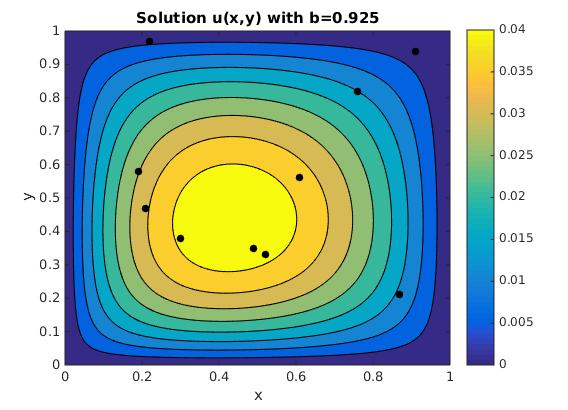
\includegraphics[scale=0.5]{./FigChap3/solu}
\caption{Numerical solution of the system (\ref{eqntoyproblem}) using a finite difference scheme. The mesh
size used in $x$ and $y$ was $0.01$. The value of the parameter $b$ was set at $0.925$. The black dots
in the plot represent the points used to generate the synthetic data about the experimental
measures $m$.}
\label{figsolU}
\end{figure}


At this point  we use the concept of emulator as in the previous chapter. If we had unlimited computational
power or time then we can run the finite difference scheme used to obtain Figure \ref{figsolU} with
a huge set of possible values for $b$ in the interval $(0,2]$. And pick the value that replicates the
better the syntetic data $m$. Since we do not have unlimited computational power or time what we
are going to do is to pick some $n$  values $b_{k}\in (0,2], k=1,2,\ldots,n$, run the finite difference
scheme on those and then use an emulator $\hat{f}$ with GPs to fill the missing data. The criteria to 
choose the number $n$ comes from considerations of how much time and computational resources we have.
For this case we chose $n=10$. How to distribute those 10 points in the interval $(0,2]$. Here we
use the concept space filling design. In the one dimensional setting it is not hard to see that
a maximin design gives an equal spacing of the 10 points in the interval $(0,2]$ hence we choose
\begin{equation*}
b_{k}=0.2k \qquad\text{for }k=1,2,\ldots,10.
\end{equation*}

We are ready to run the emulator $\hat{f}$ for these values of $b$, get a numerical value at
the 10 points in the domain where the synthetic data were created (black dots in Figure \ref{figsolU})
and use GPs to fill the missing information. Take into account that this process of `filling the blanks'
has to be done in all of the 10 measurement points in the domain $\Omega$ of definition of the phyiscal model.

In Figure \ref{fignofitted} we can see the results from running the emulator (black dots) compared
with the experimental measurement for each of the 10 sites (black line).

\begin{figure}[H]
\centering
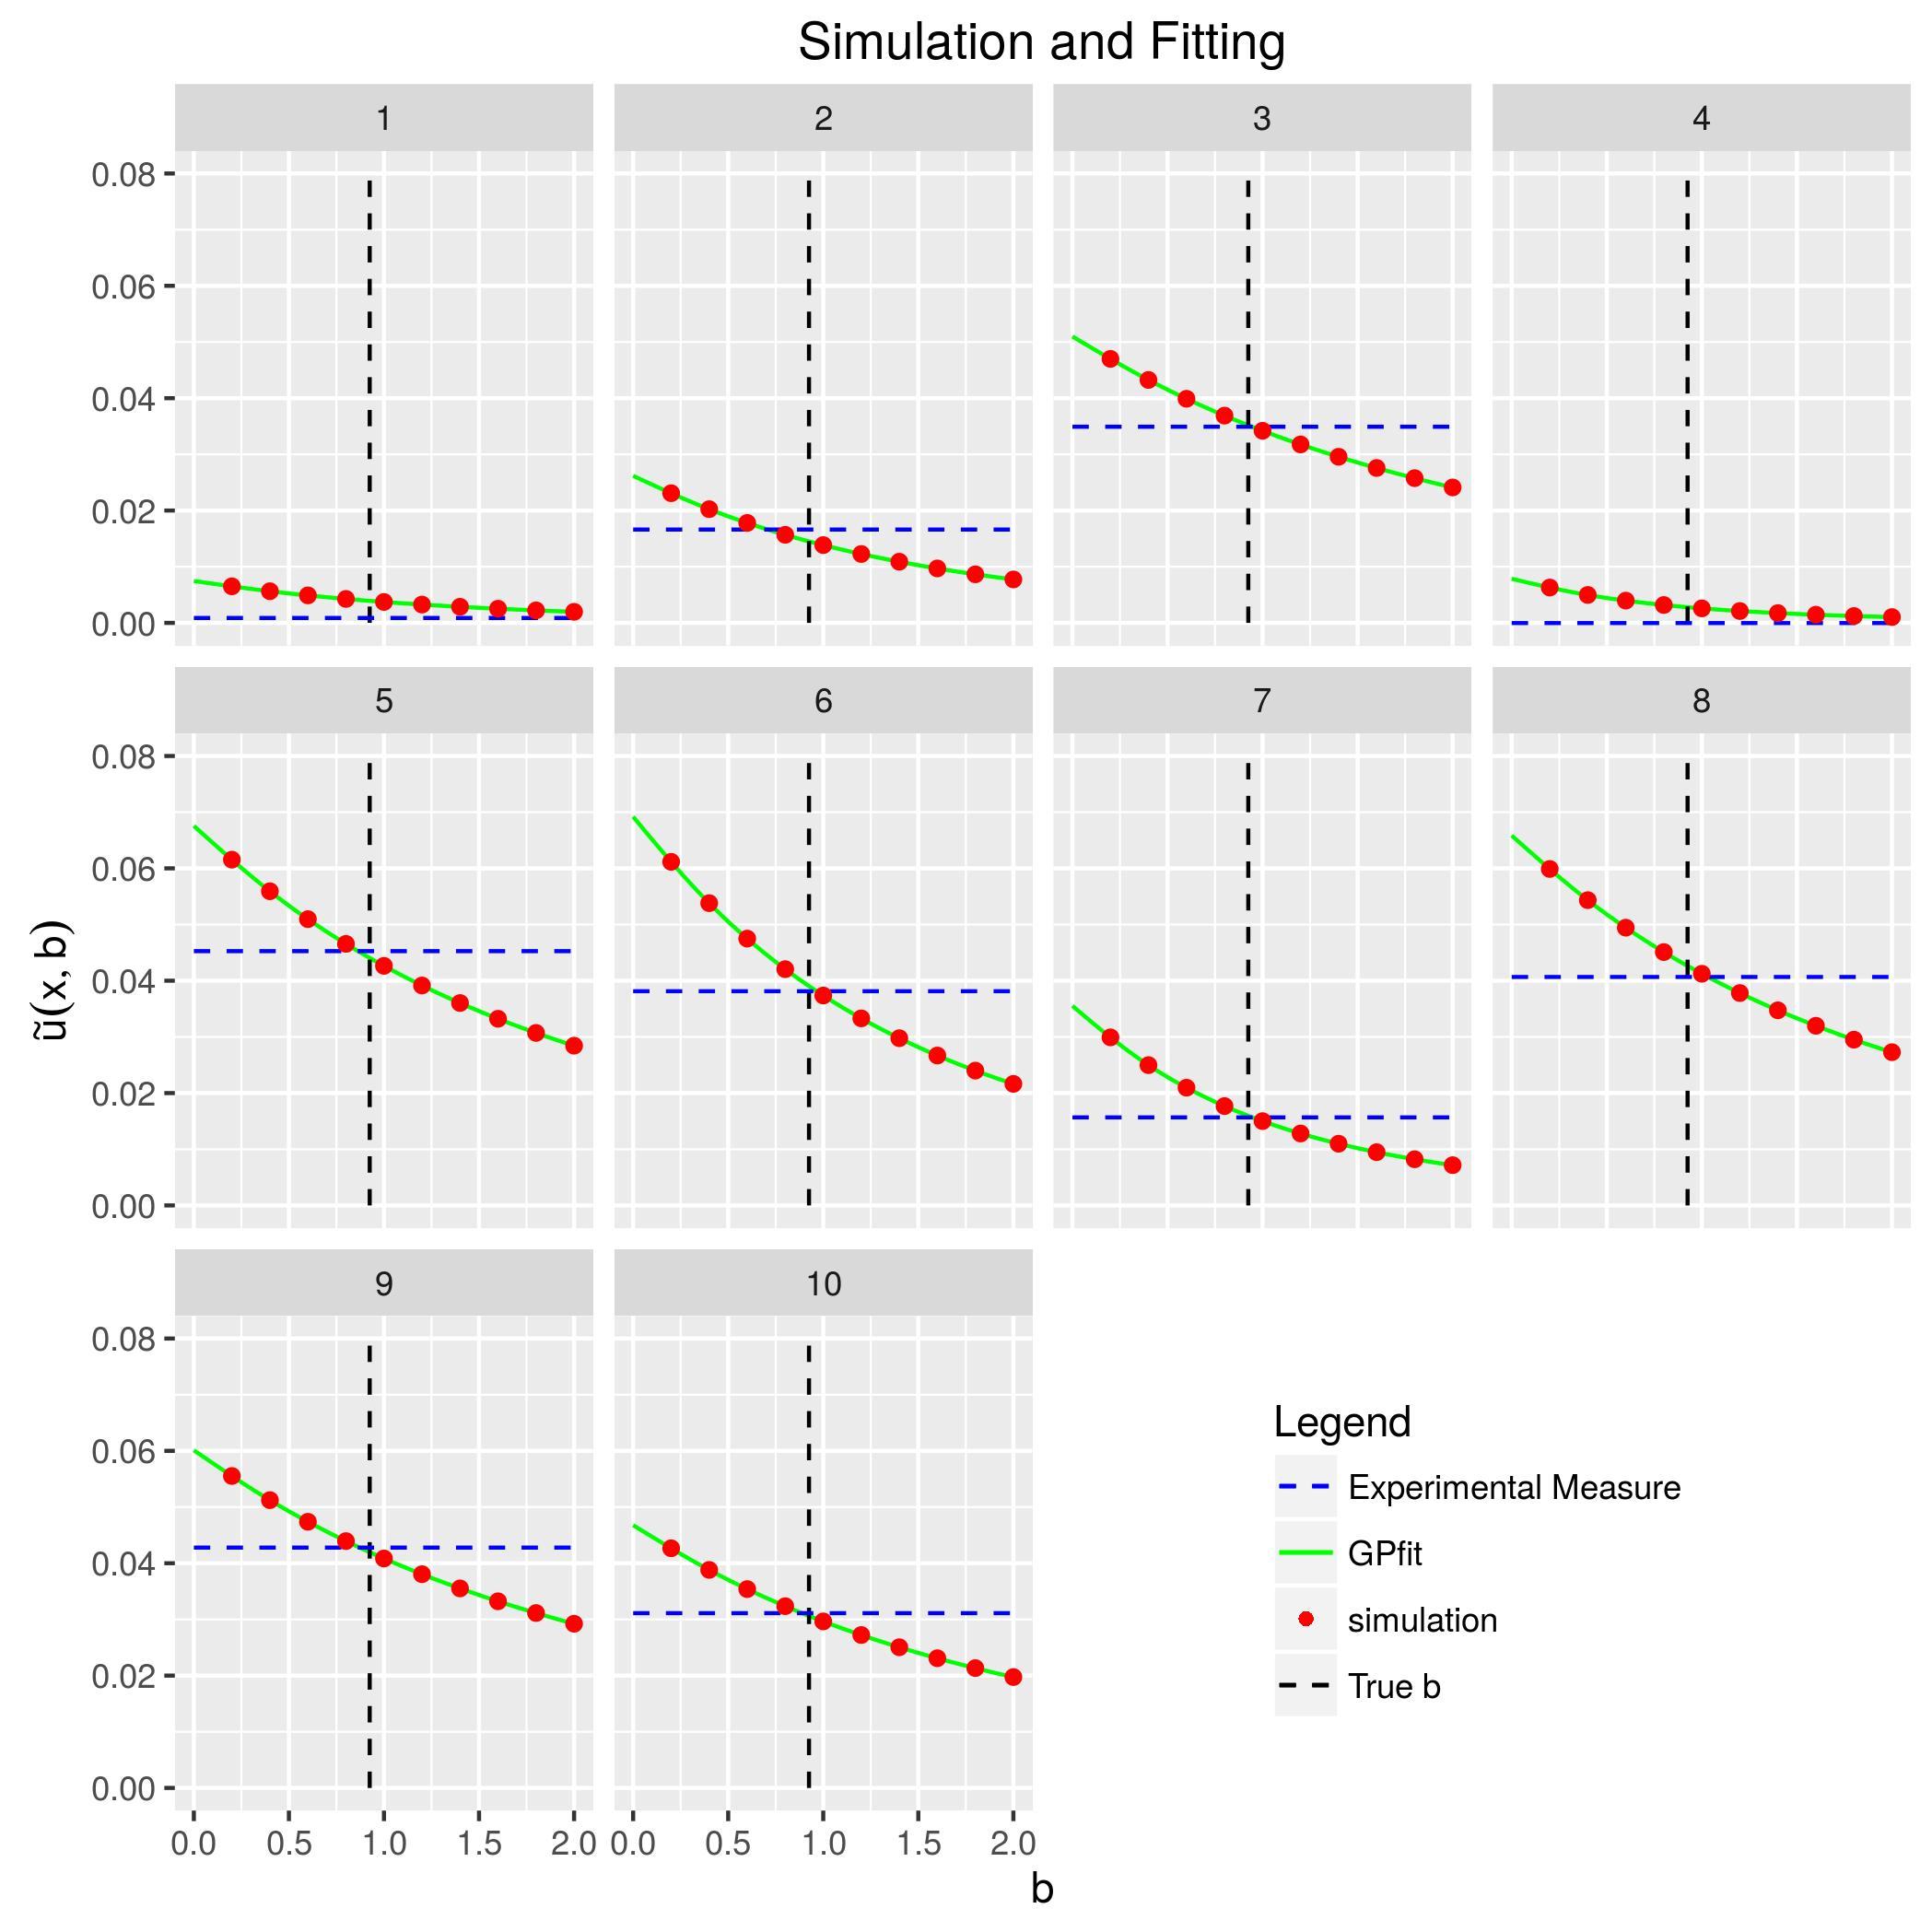
\includegraphics[scale=0.7]{./FigChap3/fitted}
\caption{whatever}
\label{fignofitted}
\end{figure}

As we can see in Figure \ref{fignofitted}, the emulator sometimes overestimates the value of $b$ and sometimes
underestimates it, this behaviour is expected. The hope is that this inaccuracies oscilate around the true
value of $b$.

Since we only have a limited number of prediction of the emulator for different values of $b$ (black points
in Figure \ref{fignofitted}), we would like to extrapolate/interpolate those results to get
more data and with that extra data, assess the value of $b$. As explained in Chapter 2, one very useful 
way to obtain the extra data is through Gaussian processes. Using the language of the previous chapter
what we want to do is, having the training points $\{(x_{i},f(x_{i})\}_{i=1}^{10}$ we want to predict 
the value of different test points $x_{i}^{*}$. This prediction is shown as a red line in Figure
\ref{fignofitted}.  The GP fit allows us to approxiamte as much value as we want, along with the uncertainty
associated with the prediction. Having this data we can now proceed to use the Bayesian methodology.
The idea goes as follows. if we denote the GP fit at at point $b$ as  $G(b)$, then we may assume
an additive noise model for the output $y$ as
\begin{equation}\label{eqnadditivenoise}
y=G(b)+\vec{\epsilon}.
\end{equation}
$\vec{\epsilon}$ is a random vector distributed as $\vec{\epsilon}\sim\mathscr{N}(0,\sigma I)$. Where $sigma=bla$
and $I$ is the $10\times 10$ identity matrix.
In the Bayesian framework we are interest in finding the value of $b$ given the experimental measurements $m$.
To that end we go back to the begining of this chapter and use equation (\ref{eqnpropto}). To use this equation
we need to find the likelihood $\like(m|b)$. Under the assumption of the additive noise model in equation
(\ref{eqnadditivenoise}) we get as in the smashed window example in chapter 2 that
\begin{equation*}
m|b\sim\mathscr{N}(G(b),\sigma I),
\end{equation*}
more precisely
\begin{equation*}
\like(m|b)=\frac{1}{(2\pi\sigma)^{n/2}}\exp\left(-\frac{\|G(b)-m\|_{2}^{2}}{2\sigma^{2}}\right).
\end{equation*}



Now we need to choose a prior for $b$. This is a delicate issue and a polemic one in the Statistics community.
The prior should reflect all of our current knowledge about $b$. However your knowledge about $b$ might be 
different than my knowledge about $b$, hence your prior for $b$ might look different than mine. For
the moment  we won't worry about that. Let's assume that our prior for $b$ is given by
\begin{equation*}
b\sim U(0,2).
\end{equation*}
where $U(a,b)$ is the uniform distribution in $a,b$. Putting all of this into formula (\ref{eqnpropto}) we get
\begin{equation*}
\post(b|m)\propto\chi_{[0,2]}\exp\left(-\frac{\|G(b)-m\|_{2}^{2}}{2\sigma^{2}}\right),
\end{equation*}
where $\chi_{[a,b]}$ is the indicator function of the set $[a,b]$. This equation can be 
interpreted as the update in knowledge from to prior to the posterior in the light of the
experimental data obtained represented by the likelihood. This change from prior to 
posterior is shown below.
\begin{figure}[H]
\centering
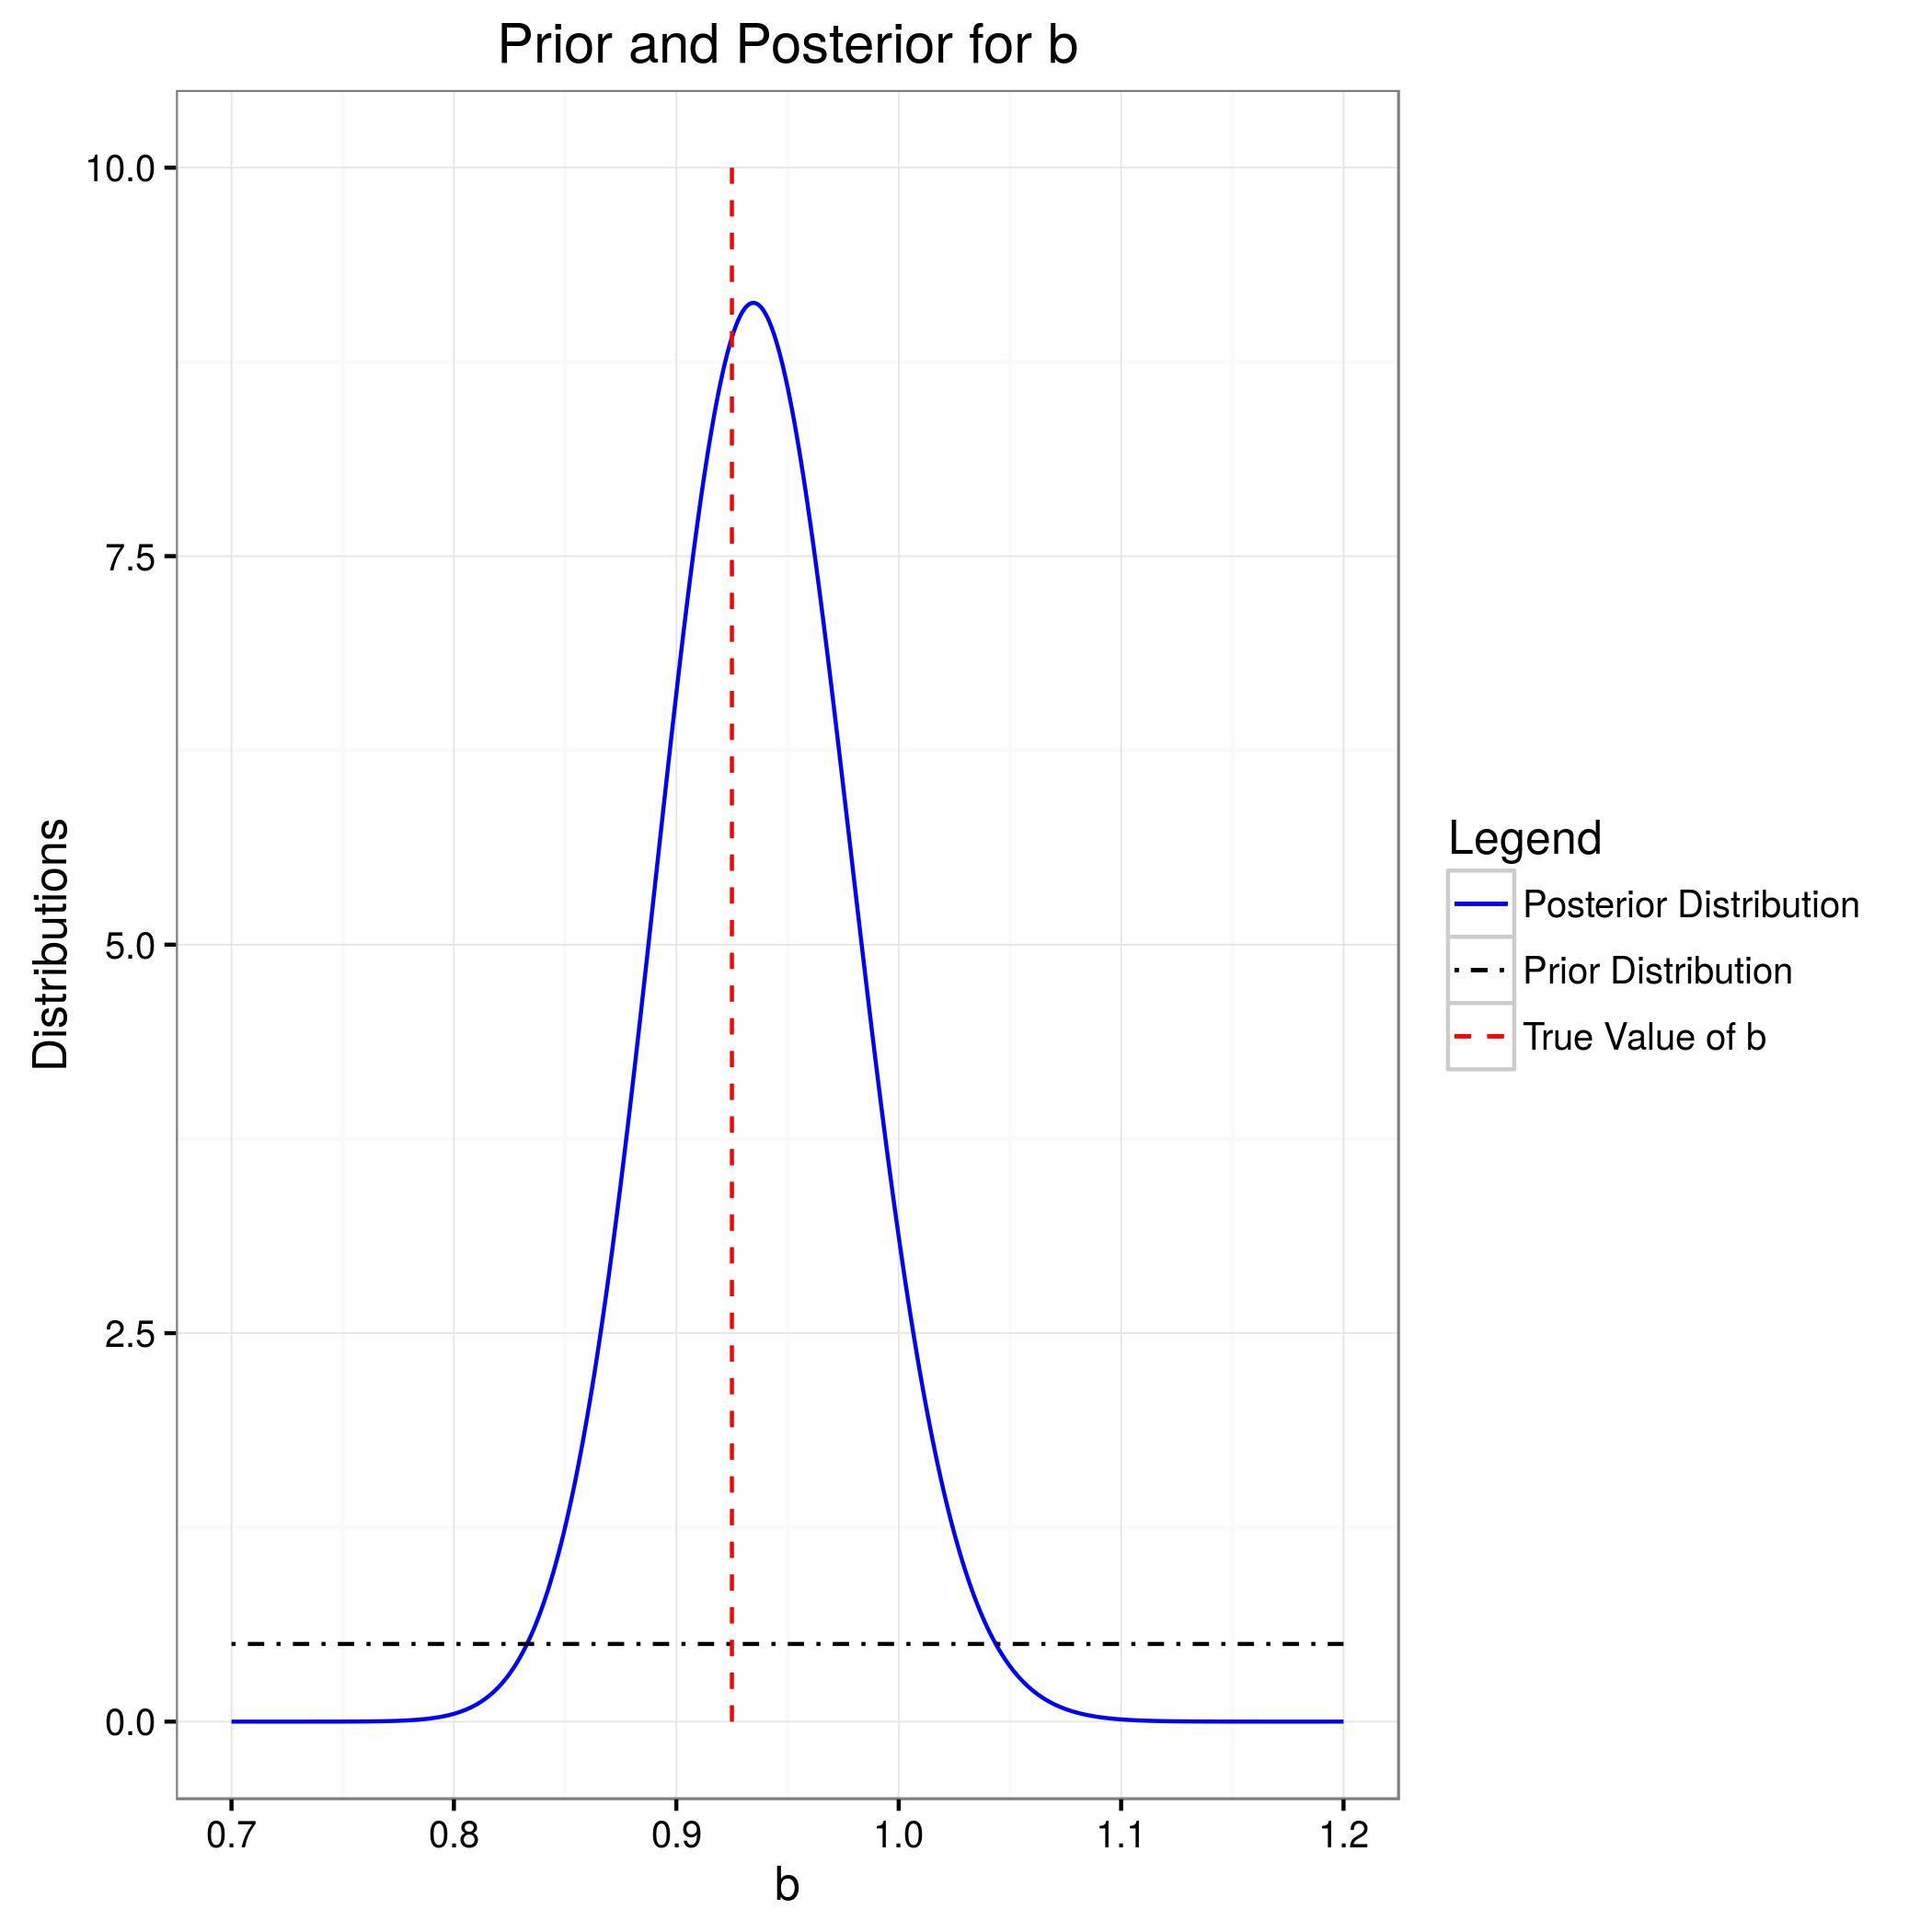
\includegraphics[scale=0.8]{./FigChap3/prior_posterior.jpg}
\caption{whatever}
\end{figure} 






As we mentioned in chapter 2,
the solution to an inverse problem in the Bayesian framework is the posterior. The question is:
how can we use this posterior to infer the value of $b$ and the uncertainty associated to it? 
\textbf{Here talk about how this integral is untractable}.

To make inferences about the value of $b$ we resort to a family of techniques from sampling probability
distributions known as Markov Chain Monte Carlo (MCMC)\textbf{Cite algun libro del MCMC}.

After using the MCMC we get the following plot 

\begin{figure}[H]
\centering
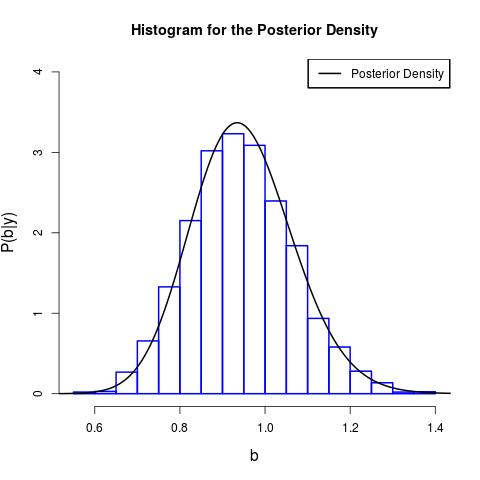
\includegraphics[scale=0.8]{./FigChap3/histogram_mcmc.jpg}
\caption{whatever}
\end{figure}



\subsection*{How important is the prior to make inferences?}
It is constructive to go in some depth and explore how prominent is the role of the prior probability
in making inferences about a problem. Let us consider the same problem as above, we want to estimate
the value of the paramter $b$. For demonstration purposes, let us assume two things. The parameter
$b$ can be any real number (not just $0<b\leq 2$ as before) and
\begin{equation*}
b\sim\mathscr{N}(b^{*},\sigma_{b}^{2}),
\end{equation*}
where $b^{*}$ and $\sigma_{b}$ are parameters to be set later.  With this new prior the formula
for the posterior becomes 
\begin{equation*}
\post(b|m)\propto \exp\left(-\frac{\|m-G(b)\|_{2}^{2}}{2\sigma^{2}}-\frac{(b-b^{*})^{2}}{2\sigma_{b}^{2}}\right).
\end{equation*}





As before, assume that the true
value of $b$ is $0.925$. To ilustrate the role that the prior has in the inference of the value
of $b$ given the experimental data $m$, let us assume that 
\begin{equation*}
b\sim\mathscr{N}(4,2.5).
\end{equation*}
That is, the person that proposed this prior is confident that within $95\%$ of confidence, the true value of
$b$ is in the interval $[1.8,8.2]$. Let us see what happens with the posterior in equation (\ref{eqnpropto})
when we get more and more experimental data. 
\begin{figure}[H]
\centering
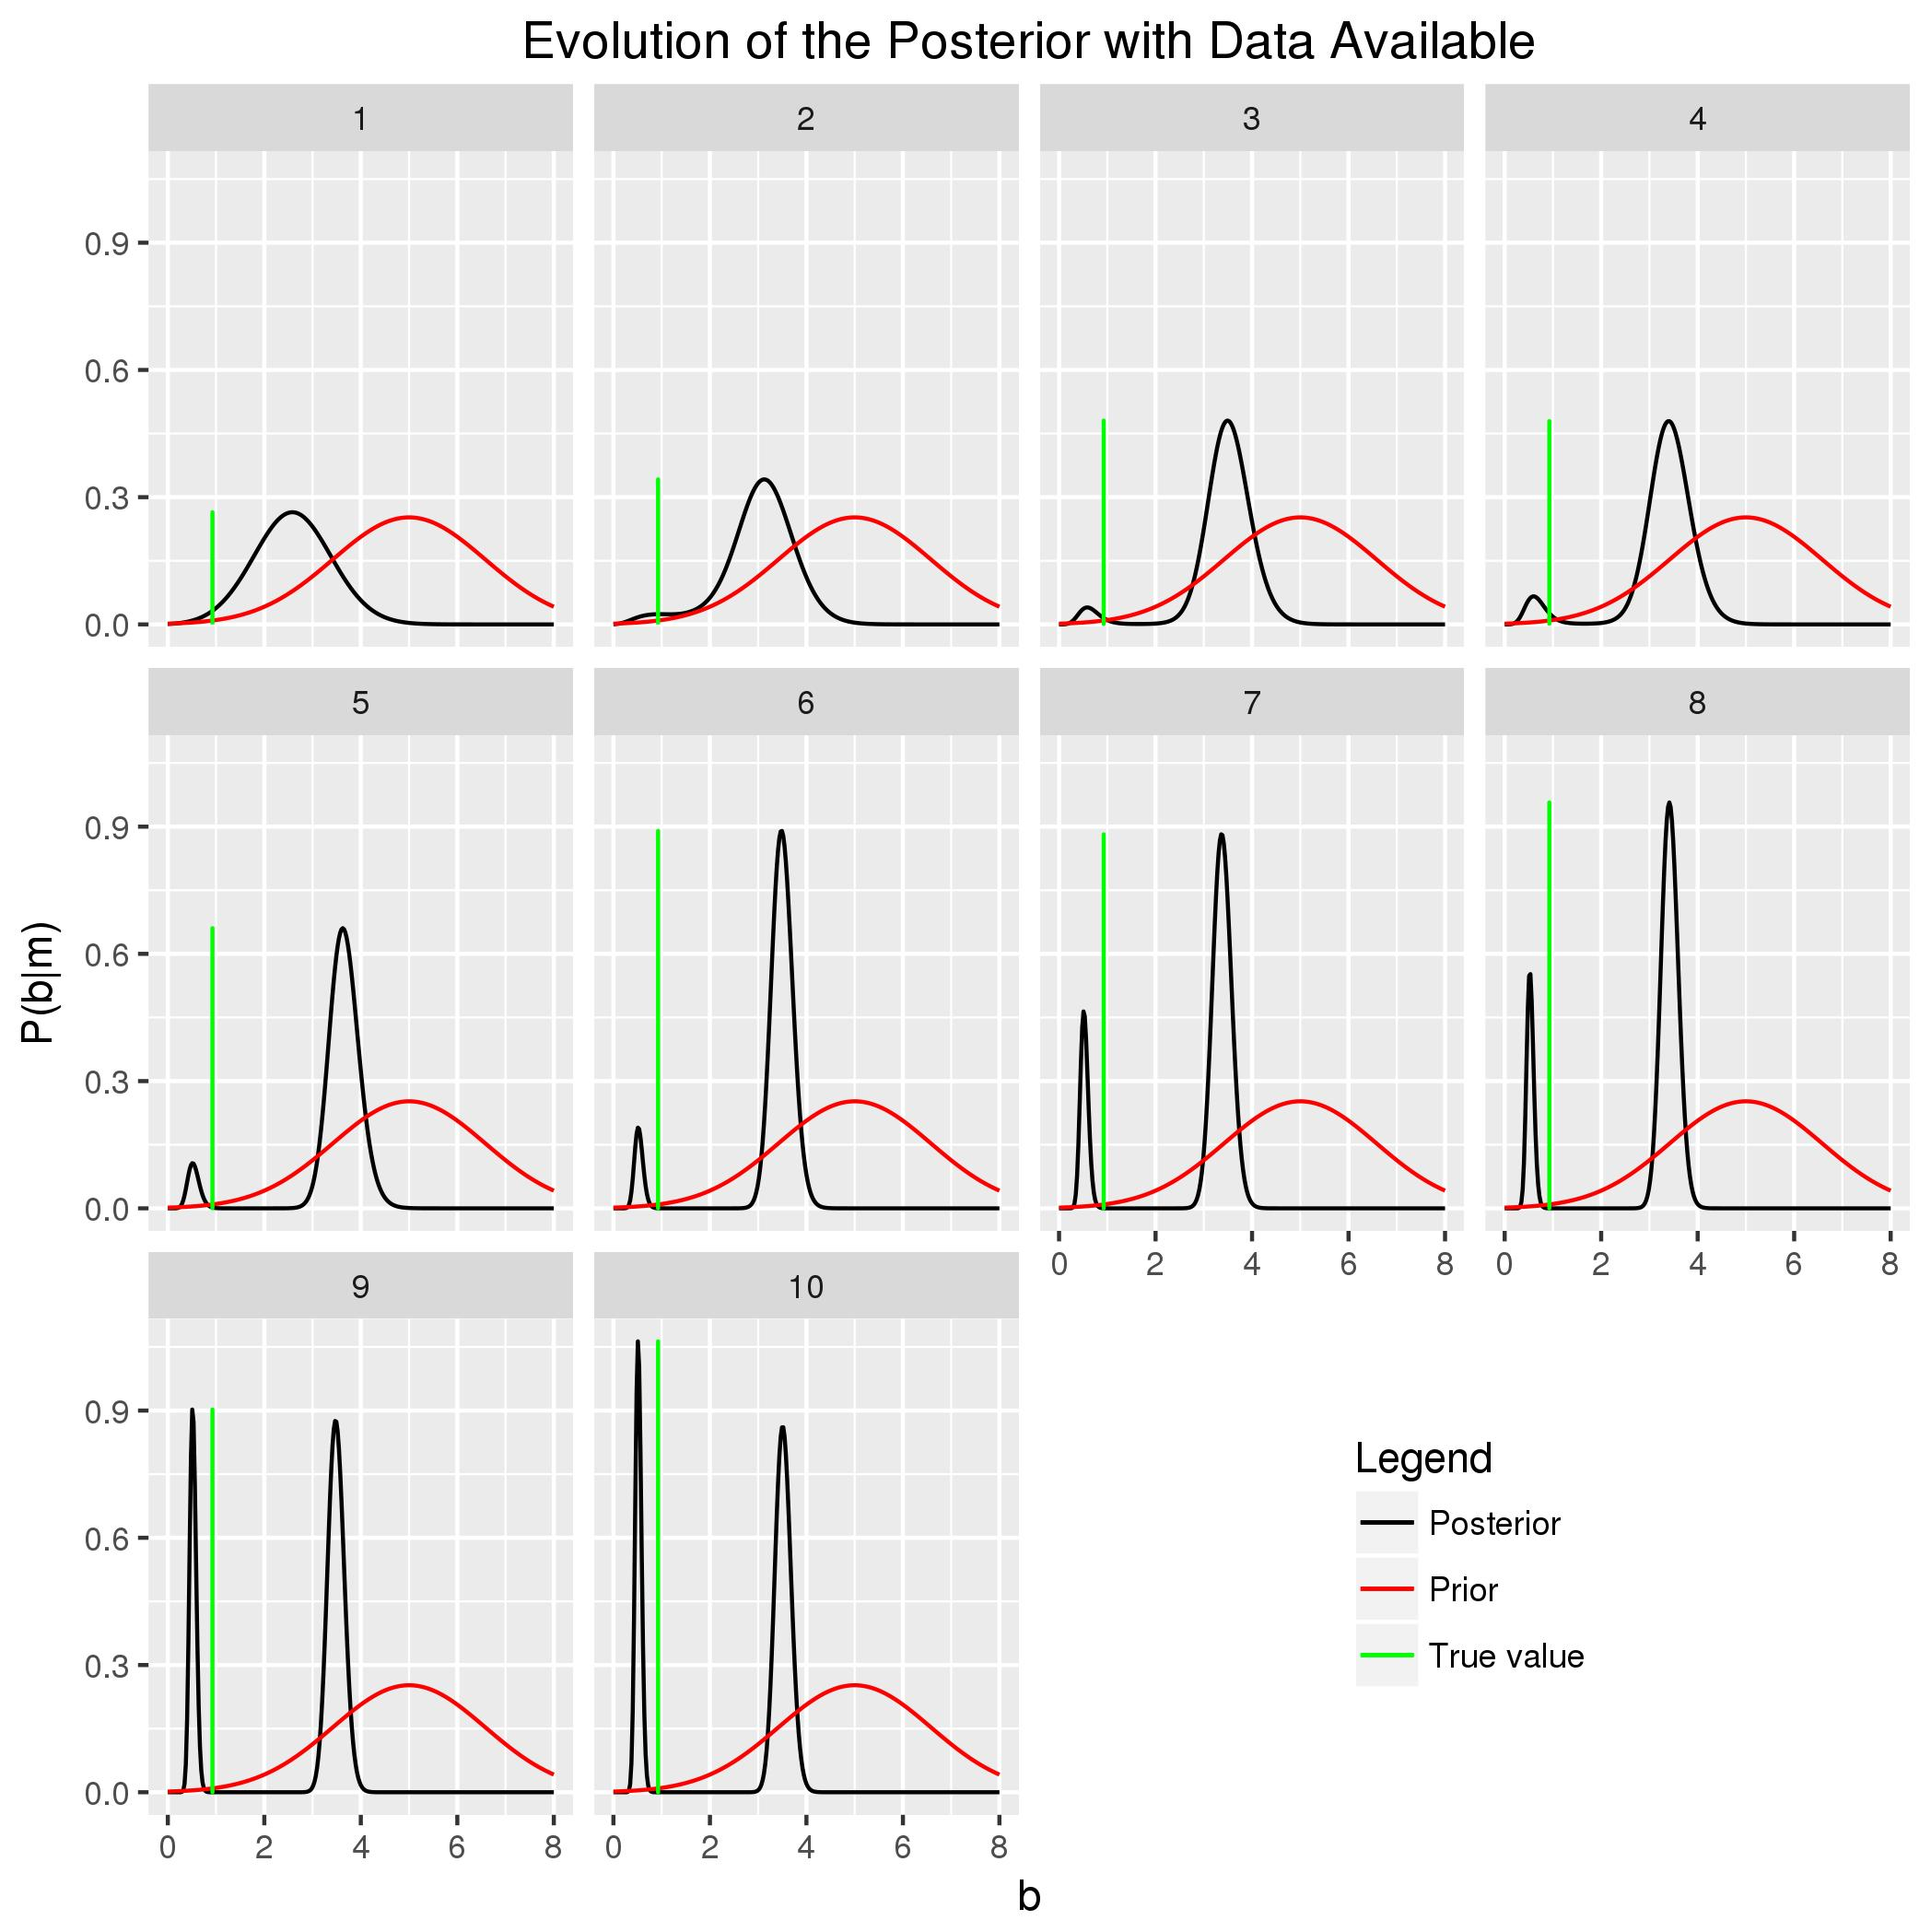
\includegraphics[scale=0.7]{./FigChap3/posterior_evolution}
\caption{bla}
\end{figure}
\bibliography{Tesis}
\bibliographystyle{plain}




\end{document}
